When we use The Lagrangian, we assume that we have:
\begin{itemize}
	\item Holonomic constraints
	\item The costraining forces do no work
	\item The applied forces are conservative
\end{itemize}
However, the potential function may change with time.

\section{D'Alembert's Principle}
From Newton's Second Law:
$$
	\dot{\bm{p}_i} = \bm{F}_i \; \rightarrow \;
	\Sigma_i (\bm{F}_i - \bm{p}_i)\cdot\delta \bm{r}_i = 0
$$
where the $\bm{r}_i$ is a virtual displacement that is consistent with the
constraints and is instantenous. We can also split the force up into the
components that are from the constraint, and those that are applied:
$$
	\bm{F}_i = \bm{F}^c_i + \bm{F}^a_i \; .
$$
As we know that the constraint forces do no work, we can simply replace the
above with the applied forces:
$$
	\Sigma_i (\bm{F}^a_i - \bm{p}_i)\cdot\delta \bm{r}_i = 0
$$
We have removed the constraint forces from this equation, but we need to rewrite
the equation in terms of the generalised co-ordinates that are
\emph{independent} of each other. This is where the proof for \emph{generalised
equations of motion (EoM)} comes in - this is in the course notes or online.
This leaves us with:
$$
	L = T - V \; \mathrm{where} \; \frac{\mathrm{d}}{\mathrm{d}t}
	\left(\frac{\partial L}{\partial \dot{q_k}}\right) - 
	\frac{\partial L}{\partial q_k} = 0\;.
$$
We can use this to solve pretty much any classical mechanics problem.
Apparently.

\subsection{Examples of the Lagrangian Method}
\paragraph{Example:} a free particle in 3D space:
$$
	T = \frac{1}{2}mv^2 = \frac{1}{2} m (\dot{x}^2 + \dot{y}^2 + \dot{z}^2)
$$
There is no potential (as the particle is free):
$$
	L = T - V = T = \frac{1}{2} m (\dot{x}^2 + \dot{y}^2 + \dot{z}^2)
$$
Putting this into the Euler-Lagrange equation:
$$
	\frac{\mathrm{d}}{\mathrm{d}t}
	\left(\frac{\partial L}{\partial \dot{q_k}}\right) - 
	\frac{\partial L}{\partial q_k} = 0\;.
$$
For each $q_k$ the answer is the same, so we will give a generalised one for
$x$, $y$, $z$:
$$
	j = \frac{\mathrm{d}}{\mathrm{d}t} (m \dot{j}) - 0 = 0
	\; \rightarrow \;
	m \ddot {j} = 0 \; ,
$$
giving the equation of motion:
$$
	j(t) = \dot{j}(0)t + j(0) \; .
$$
We also get a similar answer for constant potentials.

\subsubsection{Ignoreable co-ordinates}
If we have no explicit dependence on a co-ordinate, it can saftley be ignored
in the final E-L calculation (i.e.
$$
	\frac{\partial L}{\partial q_k} = 0\; ).
$$
If a co-ordinate is not in the Lagrangian, it is a constant which returns a 
`constant of the motion':
$$
	p_k = \frac{\partial L}{\partial \dot{q}_k}
$$
which is the conjugate momentum. For example, in the above:
$$
	\frac{\partial L}{\partial \dot{x}} = m\dot{x} = p = \mathrm{constant}
$$

\clearpage

\paragraph{Example:} a plane pendulum.
\begin{figure}[!hbt]
	\centering
	\includegraphics[width=0.25\textwidth]{PlanePendulum.png}
\end{figure}

Here, we only need one generalised co-ordinate, $\theta$, which describes how
far away the pendulum is from it's lowest point. We assume the gravitational
field is approximately constant.
$$
	T = \frac{1}{2}mv^2 = \frac{1}{2}m\left(\ell \dot{\theta}\right)^2
$$
$$
	V = mgh = mg\ell(1 - cos\theta)
$$
Giving us:
$$
	L = \frac{1}{2}m\left(\ell \dot{\theta}\right)^2 - 
	mg\ell(1 - cos\theta)
$$
Using Euler-Lagrange for $q_1 = \theta$:
$$
	\frac{\mathrm{d}}{\mathrm{d}t} \left(m \ell^2 \dot{\theta}\right) +
	mg\ell \sin \theta = 0
$$
Cancelling:
$$
	\ddot{\theta} = -\frac{g}{\ell}\sin\theta
$$
Now we use the small-angle approximation:
$$
	\ddot{\theta} = -\frac{g}{\ell}\theta
$$
Which is SHM with $\omega = \sqrt{g/L}$.

